\documentclass[12pt, letterpaper]{article}
\usepackage[utf8]{inputenc}
\usepackage{graphicx}
\usepackage{floatrow}
\usepackage{multicol}

\graphicspath{ {./images/}}

\title{Classic Cocktails}

\begin{document}

\maketitle

\pagebreak
\section{Margarita}
The Margarita is one of the most popular cocktails in North America—for good reason.
Combining the tang of lime and the sweetness of orange liqueur with the distinctive strength of 
tequila, the classic Margarita strikes all of the right keys.

\subsection*{Ingredients}

\begin{multicols}{2}

\begin{tabular} { r | l}
    15ml & Lime Juice \\
    20ml & Triple Sec \\
    50ml & Tequila \\
    pinch & Salt
\end{tabular}

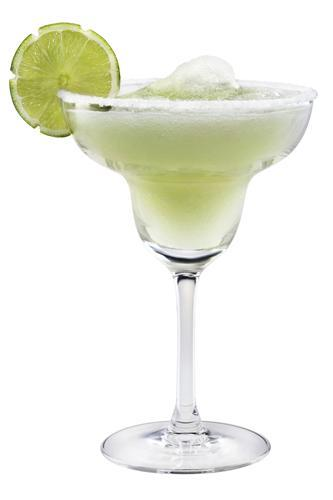
\includegraphics[height=6cm]{margarita}

\end{multicols}


\subsection*{Method}
Rim the edge of a cocktail glass with salt by coating the edge with lime juice and dipping into the salt.
Add the other ingredients to a cocktail shaker with a few cubes of ice.
Shake well for 10-15 seconds or until the outside of the shaker becomes frosted.
Strain into a cocktail glass and serve.

\pagebreak
\section{Fitzgerald}
The Fitzgerald was invented by Dale Degroff in the 1990s. Starting in the early 90s at the Rainbow Room,
New York, Mr DeGroff was instrumental in the revival and expansion of the American bar scene.
His advocacy for using fresh juices in drinks helped revitalise bars into using fresh ingredients instead of bottled sweetened juices.

\subsection*{Ingredients}

\begin{multicols}{2}

\begin{tabular} { r | l}
    25ml & Lemon Juice \\
    15ml & Simple Syrup \\
    2 dashes & Angostura Bitter \\
    50ml & Dry Gin
\end{tabular}

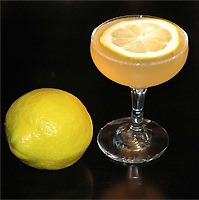
\includegraphics[height=6cm]{fitzgerald}

\end{multicols}


\subsection*{Method}
Add all ingredients to a cocktail shaker with ice and shake well.
Strain into a chilled cocktail glass. Garnish with a lemon wedge and serve.

\pagebreak
\section{Bahia}
This white rum-based crowd pleaser is made with 3 other ingredients: pineapple juice, coconut cream, cream.
\subsection*{Ingredients}

\begin{multicols}{2}

\begin{tabular} { r | l}
    90ml & Pineapple Juice \\
    75ml & White Rum \\
    15ml & Coconut Cream
\end{tabular}

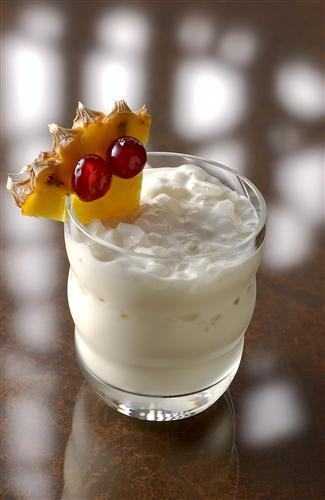
\includegraphics[height=6cm]{bahia}

\end{multicols}

\subsection*{Method}
Add all ingredients to a blender with ice and blend until smooth. Pour into a highball glass.
Garnish with a pineapple wedge, a maraschino cherry and a mint sprig, and serve.

\end{document}